\documentclass[tikz,border=5pt]{standalone}
\begin{document}

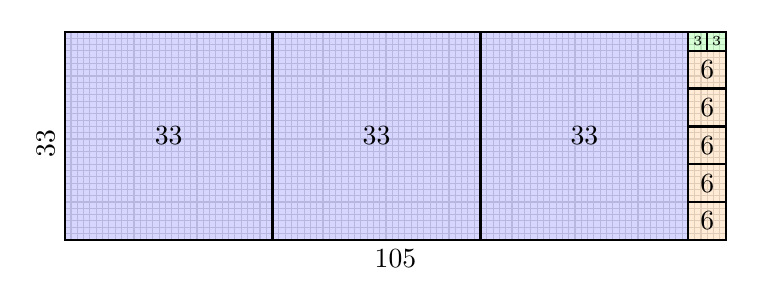
\begin{tikzpicture}[scale=0.08]

% Grid
\draw[step=1,gray!40,thin] (0,0) grid (105,33);

% Rechteck
\draw[thick] (0,0) rectangle (105,33);

% drei Quadrate 33x33 (leicht transparent)
\fill[blue!40,fill opacity=0.4] (0,0) rectangle (33,33);
\draw[thick] (0,0) rectangle (33,33);

\fill[blue!40,fill opacity=0.4] (33,0) rectangle (66,33);
\draw[thick] (33,0) rectangle (66,33);

\fill[blue!40,fill opacity=0.4] (66,0) rectangle (99,33);
\draw[thick] (66,0) rectangle (99,33);

% five quadrats 6x6 (leicht transparent)
\fill[orange!40,fill opacity=0.4] (99,0) rectangle (105,6);
\draw[thick] (99,0) rectangle (105,6);

\fill[orange!40,fill opacity=0.4] (99,6) rectangle (105,12);
\draw[thick] (99,6) rectangle (105,12);

\fill[orange!40,fill opacity=0.4] (99,12) rectangle (105,18);
\draw[thick] (99,12) rectangle (105,18);

\fill[orange!40,fill opacity=0.4] (99,18) rectangle (105,24);
\draw[thick] (99,18) rectangle (105,24);

\fill[orange!40,fill opacity=0.4] (99,24) rectangle (105,30);
\draw[thick] (99,24) rectangle (105,30);

% two quadrats 3x3 (leicht transparent)
\fill[green!40,fill opacity=0.4] (99,30) rectangle (102,33);
\draw[thick] (99,30) rectangle (102,33);

\fill[green!40,fill opacity=0.4] (102,30) rectangle (105,33);
\draw[thick] (102,30) rectangle (105,33);

% Beschriftungen der Seiten
\node[below] at (52.5,0) {105};
\node[left,rotate=90] at (-3,19) {33};
\node at (16.5, 16.5) {33};
\node at (49.5, 16.5) {33};
\node at (82.5, 16.5) {33};
\node at (102, 3) {6};
\node at (102, 9) {6};
\node at (102, 15) {6};
\node at (102, 21) {6};
\node at (102, 27) {6};
\node at (100.5, 31.5) {\tiny 3};
\node at (103.5, 31.5) {\tiny 3};

\end{tikzpicture}

\end{document}



6 = 105 - 3*33

If 6 would divide 33 (i.e.\ 6 \% 33 = 0), it would divide both, 33 and 105! However, it does not...

However, 3 = 33 - 5*6, and 3 divides 6. So, 3 also divides 3 + 5*6 = 33. So, 3 also divides 3*33 + 6 = 105. 


For the explanation of the algorithm, observe the following: (For simplicity, we assume that $a < b$, otherwise we can swap $a$ and $b$.)
$$ c | a,b \iff c | b \% a, a $$
In order to see this, first note that $c | a,b \iff c | a, (b - da)$ for any $d \neq 0$. Then, the result follows from choosing $d = b \\ a \geq 1$ since $b - (b // a) * a = b \% a$.

For a more graphical illustration, consider a rectangle with side lengths $a$ and $b$. Finding $gcd(a,b)$ is equivalent to finding the largest square that can fit into this rectangle without leaving any leftover space.

We can cut out squares of side length $a$ from the rectangle, and we are left with a smaller rectangle with side lengths $a$ and $b \% a$. The common divisors of $a$ and $b$ are exactly the common divisors of $a$ and $b \% a$, since any common divisor of $a$ and $b$ must also be a common divisor of $a$ and the leftover part after cutting out the squares, and vice versa.: 


Indeed, if $c$ divides $a$ and $b$, then it also divides any linear combination of $a$ and $b$, in particular, it divides $b - (b // a) * a = b \% a$. Conversely, if $c$ divides $a$ and $b \% a$, then it also divides any linear combination of $a$ and $b \% a$, in particular, it divides $(b // a) * a + b \% a = b$.


a < b
gcd(a,b) = gcd(b \% a, a)

c | a,b 

c | b \% a, a => c | (b // a) * a + b \% a = b

c | a,b => c | (b - (b // a) * a) = b \% a

